\documentclass[UTF8]{ctexart}
\usepackage{geometry}
\usepackage{graphicx}
\usepackage{latexsym,bm,amsmath,amssymb}
\geometry{a4paper,scale=0.8}
\title{Bayes}
\author{AsukaShiKi}
\date{\today}
\begin{document}
\maketitle
\par
\begin{figure}[ht]
    \centering
    
\includegraphics[scale=1.3]{01.jpg}
\end{figure}
\begin{figure}[ht]
    \centering
    
\includegraphics[scale=0.3]{02.jpg}
\end{figure}
\newpage
\tableofcontents
\newpage
\Large{
\section{贝叶斯分类器}
贝叶斯分类器是一种最大化后验概率进行单点估计的分类器。本章内容大致如下:\par
1.贝叶斯决定论:如何计算某个样本误分类的期望损失/条件风险?贝叶斯判定准则是怎样的?
什么是判别式模型?什么是生成式模型?贝叶斯定理中各个概率代表什么?估计后验概率有什么
难处?\par
2.极大似然估计:如何估计条件概率?频率学派和贝叶斯学派对参数估计有什么不同的见解?
极大似然估计的思想是什么?如何处理概率连乘造成的下溢?试想一下连续属性和离散属性的
极大似然估计。这种估计方法有什么缺点?\par
3.朴素贝叶斯分类器:朴素贝叶斯分类器是基于什么假设的?表达式怎么写?为什么估计概率
值时需要进行平滑?拉普拉斯修正是怎样的?现实任务中中如何使用朴素贝叶斯分类器?\par
4.半朴素贝叶斯分类器:半朴素贝叶斯分类器是基于什么假设的?什么是独依赖估计?独依赖
分类器有哪些学习方法?AODE有什么优点?是否可以通过考虑属性之间的高阶依赖来进一步提
升模型的泛化性能?\newpage
\section{贝叶斯决策论}
\subsection{后验概率}
后验概率是指在得到结果的基础上,执果寻因;即事情已经发生,要求这件事发生的原因是由某
个因素引起的可能性的大小,就是后验概率。\par
后验概率的计算需要使用贝叶斯公式:
\begin{center}
    \Large{
        $P(B_i|A)=\frac{P(A|B_i)P(B_i)}{\sum_{i=1}^nP(A|B_i)P(B_i)}$\\[2ex]
    }
\end{center}
其中$P(B|A)$是在$A$发生的情况下$B$发生的可能性。$B_1,B_2,B_3,....,B_n$是完备事件组,即
$\cup_{i=1}^nB_i=\Omega,B_iB_j=\phi,P(B_i)>0$。
\subsection{贝叶斯决策论}
贝叶斯决策论(Bayesian decision theory)是概率框架下实施决策的基本方法。具体来说,
在分类任务中,贝叶斯决策论基于概率和误判损失选择出最优的类别标记。\par
若将上一节样本空间中的划分$B_i$看作是类标,$A$看作是一个新的样本,很容易将条件概率理解
为样本$A$是类别$B_i$的概率。\par
假设有$N$种可能的标记,即$\mathcal Y={c_1,c_2,c_3,...,c_N,\lambda_{ij}}$是将一个真实
标记为$c_j$的样本误分类为$c_i$所产生的损失。基于后验概率$P(c_i|x)$可获得将样本$x$分类为
$c_i$所产生的期望损失,即在样本$x$上的“条件风险”:
\begin{center}
    \Large{
        $R(c_i|x)=\sum\limits_{j=1}\limits^N\lambda_{ij}P(c_j|x)$
    }
\end{center}
我们的任务就是寻找一个判定准则最小化所有样本的条件风险总和,因此就有了贝叶斯判定准则
(Bayes decision rule):为最小化总体风险,只需在每个样本上选择那个使得条件风险最小的
类标。
\begin{center}
    \Large{
        $h^*(x)=arg\min\limits_{c\in\mathcal Y}R(c|x)$
    }
\end{center}\par
这个判断准则$h^*$称为贝叶斯最优分类器,对应的总体风险$R(h^*)$称为贝叶斯风险,而$1-R(h^*)$
则反映了分类器所能达到的最好性能,也即模型精度的理论上限。\par
进一步的,如果我们学习模型的目标是令分类错误率最小,那么分类正确时误分类$\lambda_{ij}$损失
为0,反之为1,即:
\Large{
    $$\lambda_{ij}=\left\{
        \begin{aligned}
            0,&&if \quad i = j;\\
            1,&&otherwise;
        \end{aligned}
        \right.
        $$
}
这时条件风险就是:
\begin{center}
    $R(c|x)=1-P(c|x)$
\end{center}
于是,最小化分类错误率的贝叶斯最优分类器为:
\begin{center}
    $h^*(x)=arg\max\limits_{c\in\mathcal Y}P(c|x)$
\end{center}
若要风险最小,我们只需要选择使样本$x$后验概率最大的类别标记即可。那么,我们的问题就转化为获取
后验概率。\par
事实上,从概率的角度理解,机器学习的目标就是基于有限的训练样本尽可能准确的估计出后验概率,要
实现这个目标,主要有两种策略:\\[2ex]
1.构建判别式模型:给定样本$x$,直接对后验概率$P(x|c)$建模来预测$c$。这类模型包括有决策树,BP
神经网络,支持向量机等。\\[2ex]
2.构建生成式模型:给定样本$x$,先对联合概率分布$P(x,c)$建模,然后再利用联合概率计算出后验概率
$P(c|x)$,也即$P(c|x)=\frac{P(x,c)}{P(x)}$。\par
基于贝叶斯定理,$P(c|x)$可以写为:
\begin{center}
    \LARGE{
        $P(c|x)=\frac{P(c)P(x|c)}{P(x)}$
    }
\end{center}\par
在贝叶斯定理中,每个概率都有约定俗成的名称:\par
1.$P(c|x)$是类标记$c$相对于样本$x$的条件概率,也由于得自$x$的取值而被称作$c$的后验概率。\par
2.$P(x|c)$是样本$x$相对于类标记$c$的类条件概率(class-conditional probability),或称为似
然($likelihood$),也由于得自$c$的取值而被称作$x$的后验概率。\par
3.$P(c)$是$c$的先验概率(也称为边缘概率),之所以称为"先验"是因为它不考虑任何$x$方面的因素。在这
里又称为类先验(prior)概率。\par
4.$P(x)$是$x$的先验概率。在这里是用作归一化的证据(evidence)因子,与类标记无关。\par
有了贝叶斯定理之后,我们就可以把求取后验概率$P(c|x)$的问题转化为如何计算先验概率$P(c)$和类条件
概率$P(x|c)$。\par
类先验概率$P(c)$表示的是样本空间中,各类样本的比例,根据大数定律,当训练集包含足够多的独立同分布
样本时,类先验概率可以直接通过训练集中各类样本出现的频率进行估计。\par
类条件概率$P(x|c)$的情况相对复杂得多,它涉及到类$c$中样本$x$所有属性的联合概率,假设每个样本有$d$
个二值属性,那么可能的取值组合就多达$2^d$个,这个数目可能远多于训练集的规模,也就意味着很多样本的
取值没有在训练集中出现,所以直接用训练集出现的频率进行估计是不可行的。必须注意未被观测到和出现概率
为0的区别。\par
注意,上述讨论中,均假设属性是离散型,对于连续型属性,只需把概率质量函数$P(·)$换为概率密度函数$p(·)$
就可以了。\newpage
\section{极大似然估计}
\subsection{极大似然估计原理}
极大似然估计的原理可以用下图中的例子说明:
\begin{figure}[ht]
    \centering
    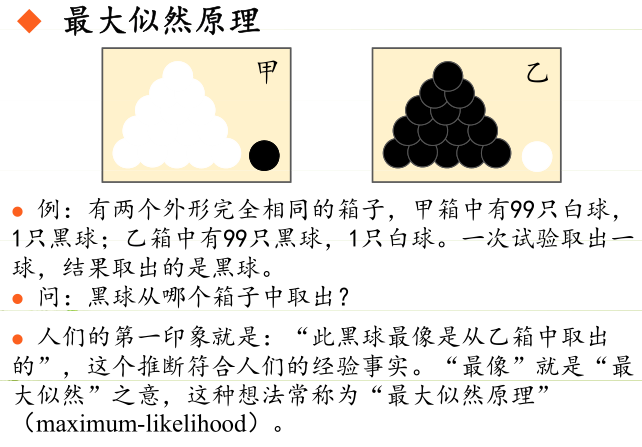
\includegraphics[scale=0.8]{03.jpg}
\end{figure}\par
总结起来,最大似然估计的目的就是:利用已知的样本结果,反推最有可能(最大概率)导致这样结果的参数值。\par
原理:极大似然估计是建立在极大似然原理的基础上的一个统计方法,是概率论在统计学中的应用。极大似然估计
提供了一种给定观察数据来评估模型参数的方法,即:“模型已定,参数未知”。通过若干次试验,观察其结果,利
用试验结果得到某个参数值能够使样本出现的概率为最大,则称为极大似然估计。\par
\subsection{极大似然估计应用到类条件概率估计}
估计类条件概率的一种常用策略是:先假定该类样本服从某种确定的概率分布形式,然后再基于训练集中的该类样
本对假定的概率分布的参数进行估计。比方说假定该类样本服从高斯分布,那么接下来就是利用训练集中该类样本
来估计高斯分布的参数——均值和方差。\par
具体来说,记关于类别$c$的类条件概率为$P(x|c)$,假设$P(x|c)$,假设$P(x|c)$具有确定的形式,并且被参数
向量$\theta_c$唯一确定,则我们的任务就是利用训练集$D$估计参数$\theta_c$。为明确起见,我们将$P(x|c)$
记作$P(x|\theta_c)$。\par
令$D_c$表示训练集$D$中第$c$类样本组成的集合,假设这些样本是独立同分布的,则参数$\theta_c$对于数据集
$D_c$的似然是:
\begin{center}
    \Large{
        $P(D_c|\theta_c)=\prod\limits_{x\in D_c}P(x|\theta_c)$
    }
\end{center}
对参数$\theta_c$进行极大似然估计,即寻找能最大化似然$P(D_c|\theta_c)$的参数值$\hat{\theta_c}$。
即,在所有$\theta_c$的可能取值中,找到使数据出现可能性最大的一个$\theta_c$值。\par
因为连乘操作容易导致下界溢出,实际应用中通常使用对数似然代替:
\Large{
    \begin{align*}
        LL(\theta_c)&=logP(D_c|\theta_c)\\[2ex]
                    &=\sum\limits_{x\in D_c}logP(x|\theta_c)
    \end{align*}
}\par
此时参数$\theta_c$的极大似然估计$\hat{\theta_c}$为:
\begin{center}
    \LARGE{
        $\hat{\theta_c}=arg\max\limits_{\theta_c}LL(\theta_c)$
    }
\end{center}\par
求解的过程就是求似然函数的导数,然后令导数为0,得到似然方程,解方程得到最优解,也即该类样本分布的
参数。\newpage
\section{朴素贝叶斯分类器}
\subsection{朴素贝叶斯分类器概念}
估计后验概率$P(c|x)$最大的难处在于:类条件概率$P(x|c)$是所有属性上的联合概率,而多个属性的不同属性值组合不一定被
训练集全部囊括,所以很难通过训练集来估计。\par
为了避开这个障碍,朴素贝叶斯分类器采用属性条件独立性假设:对已知类别,假设所有属性相互独立。即,假
设每个属性独立地对分类结果发生影响。\par
基于上述假设,可以将类条件概率写成连乘的形式,因此,贝叶斯概率可以重写为:
\begin{center}
    \LARGE{
        $P(c|x)=\frac{P(x|c)P(c)}{P(x)}=\frac{P(c)}{P(x)}\prod\limits_{i=1}\limits^dP(x_i|c)$
    }
\end{center}
其中$d$为属性数目,$x_i$为样本$x$在第$i$个属性上的取值。\par
又因为$P(x)$与类别无关,所以朴素贝叶斯分类器的表达式可以写为:
\begin{center}
    \LARGE{
        $h(x)=arg\max\limits_{c\in \mathcal Y}P(c)\prod\limits_{i=1}\limits^dP(x_i|c)$
    }
\end{center}\par
又因当训练集中包含足够多的独立同分布样本时,类先验概率$P(c)$可以直接算出,也即训练集该类样本的数目
占训练集规模的比例:
\begin{center}
    \LARGE{
        $P(c)=\frac{|D_c|}{|D|}$\quad(1)\\[2ex]
    }
\end{center}\par
而条件概率$P(x_i|c)$根据属性类型分为离散型和连续型两种情况:\par
1.离散型属性:令$D_c,x_i$表示$D_c$中在第$i$个属性上取值为$x_i$的样本组成的集合,则条件概率$P(x_i|c)$可
估计为:
\begin{center}
    \LARGE{
        $P(x_i|c)=\frac{|D_{x,x_i}|}{|D_c|}$\quad(2)\\[2ex]
    }
\end{center}\par
2.连续型属性:考虑概率密度函数,假定$p(x_i|c)\sim\mathcal N(\mu_{c,i},\sigma^2_{c,i})$\footnote{$\mathcal N$
是高斯分布},其中$\mu_{c,i}$和$\sigma^2_{c,i}$分别是第$c$类样本在第$i$个属性上取值的均值和方差,则有:
\begin{center}
    \LARGE{
        $p(x_i|c)=\frac{1}{\sqrt{2\pi}\sigma_{c,i}}exp(-\frac{(x_i-\mu_{c,i})^2}{2\sigma^2_{c,i}})$
    }
\end{center}
我们利用类别$c$的样本子集在该属性上的取值算出分布的均值和方差,然后把属性取值$x_i$代入概率密度函数就可算出这个
条件概率。
\subsection{拉普拉斯修正/平滑}
若某个属性值在训练集中没有与某个类同时出现过,那么,它对应的条件概率$P(x_i|c)$就为0。在连乘中,这就意味着整个式子
都为0,其他属性携带的信息都被抹去了。这是很常见的情况,举个例子,假设有一篇新闻应该在体育版发布的,它包含
了 “罗纳尔多” 这个词,但由于我们构造分类器时,训练集中所有 “体育” 类的文本都没有出现这个词,于是,该新闻按照重写后
的贝叶斯公式计算出的体育类的条件概率必定为0;而恰好 “娱乐” 类的文本中有一篇包含了这个词,那么计算出的娱乐类的条件
概率就大于0,从而使得这篇新闻被误分到娱乐版发布了,这显然很不合理。\par
此时,我们需要对概率值进行平滑,最常用的是拉普拉斯修正,假设训练集中包含有$N$个类别,第$i$个属性包含有$N_i$中取值,
则拉普拉斯修正把式(1)和式(2)修改为:
\begin{align*}
        P(c)&=\frac{|D_c|+1}{|D|+N}\quad(3)\\[2ex]
        P(x_i|c)&=\frac{|D_{c,x_i}|+1}{|D_c|+N_i}\quad(4)
\end{align*}
拉普拉斯修正保证了不会因为训练集样本不充分而导致概率估值为0。但它实际上是假设了类别和属性值是均匀分布的,相当于额外
引入了先验,这个假设并不总是成立。不过当训练集规模足够大时,引入先验所产生的影响会变得非常低。也可以理解为,此时式
(3)和式(4)的分母很大,使得分子中引入的1带来的变化非常小,此时概率的估计值会趋向于真实值。\newpage
\subsection{实际应用}
朴素贝叶斯分类器和前面学习的模型有一个不同的地方就是,我们并不是基于训练集和某些算法来学习模型的参数;而是利用训练
集来算出一些概率,在预测时,根据新样本的情况,使用不同的概率计算出它被分到各个类的后验概率,然后取后验概率最大的一
个类作为结果。\par
在实际任务中,有两种使用方式:\par
1.查表:若对预测速度要求较高,可以先根据训练集把所有涉及到的概率计算出来,然后存储好,在预测新样本时只需要查表然
后计算就可以了。\par
2.懒惰学习:若数据更替比较频繁,也可以理解为用训练集算出的概率可能很快就失效了,更新换代的速度很快,那就采取懒惰
学习(lazy learning)的方式,仅当需要预测时才计算涉及到的概率。\par
特别地,当我们采取了预先计算所有概率的方式时,如果有新数据加入到训练集,我们只需要更新新样本涉及到的概率(或者说计
数)就可以了,可以很方便地实现增量学习。\newpage
\section{半朴素贝叶斯分类器}
由于朴素贝叶斯分类器中采用的属性条件独立性假设在现实任务中很难成立,有时候属性之间会存在依赖关系,这时候我们就需要
对属性条件独立性进行适当的放松,适当考虑一部分属性间的相互依赖信息,从而既不需要进行完全联合概率计算,又不至于彻底
忽略了比较强的属性依赖,这就是半朴素贝叶斯分类器的基本思想。\par
“独依赖估计”(简称ODE)是半朴素贝叶斯分类器最常用的策略。所谓“独依赖”就是假设每个属性在类别之外最多依赖于一个其他属
性,即:
\begin{center}
    \LARGE{
        $P(c|x)\propto P(c)\prod\limits_{i=1}\limits^dP(x_i|c,pa_i)$\quad(5)
    }
\end{center}
其中$pa_i$为属性$x_i$所依赖的属性,称为$x_i$的父属性。此时对每个属性$x_i$,若其父属性$pa_i$已知,则可采用类似式(4)
的办法来估算概率值$P(x_i|c,pa_i)$。于是,问题的关键就转化为如何确定每个属性的父属性,不同的做法产生不同的独依赖分类
器。\par
\subsection{SPODE方法}
最直接的做法是假设所有属性都依赖于同一个属性,称为“超父”,然后通过交叉验证等模型选择来确定超父属性,由此就形成了SPODE
方法。下图中,$x_1$就是超父属性。
\begin{figure}[ht]
    \centering
    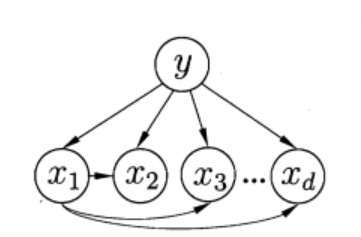
\includegraphics[scale=0.6]{04.jpg}
\end{figure}
\subsection{TAN方法}
TAN(Tree augmented naive Bayes)则是一种基于最大带权生成树(maximum weighted spanning tree)的方法,通过以下四个
步骤将属性间的依赖关系约简成下图的结构:
\begin{figure}[ht]
\centering
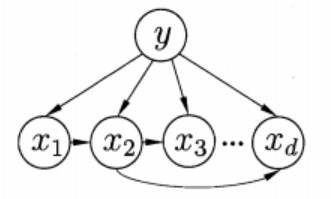
\includegraphics[scale=0.6]{05.jpg}    
\end{figure}
具体步骤如下:\par
1.计算任意两个属性之间的条件互信息。
\begin{center}
    $I(x_i,x_j|y)=\sum\limits_{x_i;x_j;c\in \mathcal Y}P(x_i,x_j|c)log\frac{P(x_i,x_j|c)}{P(x_i|c)P(x_j|c)}$
\end{center}\par
2.以属性为节点构建完全图,任意两个节点之间边的权重设为$I(x_i,x_j$\\$|y)$;\par
3.构建此完全图的最大带权生成树,挑选根变量,将边置为有向;\par
4.加入类别节点$y$,增加从$y$到每个属性的有向边。\par
条件互信息$I(x_i,x_j|y)$刻画了属性$x_i,x_j$在已知类别情况下的相关性,因此,通过最大生成树算法,TAN实际上仅保留了强相关
属性属性之间的依赖性。
\subsection{AODE}
AODE是基于集成学习机制,更加强大的独依赖分类器,与SPODE通过模型选择确定超父属性不同,AODE尝试将每个属性做为超父来构建SPODE,
然后将具有足够数据支撑的SPODE集成起来作为最终结果,即:
\begin{center}
    $P(c|x)\propto\sum\limits_{i=1,|D_{x_i}|\geq m^{'}}\limits^dP(c,x_i)\prod\limits_{j=1}\limits^dP(x_j|c,x_i)$
\end{center}
其中$D_{x_i}$是在第i个属性上取值为$x_i$的样本的集合,$m^{'}$为阈值常数,AODE需要估计$P(c,x_i)$和$P(x_j|c,x_i)$.类似式4,
有:
\begin{align*}
    \hat{P}(c,x_i)&=\frac{|D_{c,x_i}|+1}{|D|+N_i}\\[2ex]
    \hat{P}(x_j|c,x_i)&=\frac{|D_{c,x_i,x_j}|+1}{|D_{c,x_i}|+N_j}
\end{align*}
其中$N_i$是第i个属性可能的取值数,$D_{c,x_i}$是类别为c且在第i个属性上取值为$x_i$的样本集合,$D_{c,x_i,x_j}$是类别为c且在
第i和第j个属性上取值分别为$x_i$和$x_j$的样本集合。\\
finished at 27/2/2019
}
\end{document}